\documentclass[journal]{IEEEtran}
\usepackage{booktabs,graphicx,amsmath,xcolor,url}
\usepackage[hidelinks]{hyperref}
\usepackage{cite}

\begin{document}

\title{A One-Way Ratchet: Seven Years of Change in AWS Managed IAM Policies}

\author{Mithil~Nagabathula%
\thanks{M. Nagabathula is with the School of Architecture, Computing and Engineering, University of East London, London E16 2RD,
United Kingdom (e-mail: mithilnishu2000@gmail.com). ORCID: 0009-0005-1722-1138.}}

\markboth{Manuscript submitted to IEEE Access}{Nagabathula: A One-Way Ratchet}

\maketitle

\begin{abstract}
AWS managed policies are permission sets written and maintained by AWS and attached by customers to their own identities. When AWS
edits one, every attachment changes at once without customer action. We analyse a public archive that has recorded every managed
policy daily since February 2019 (1{,}669 policies, 11{,}107 recorded modifications). Policies grew from 515 to 1{,}667 and listed
actions 6.6-fold. Of 2{,}992 modifications that changed which actions a policy grants, 91\% only added actions; 28{,}632 grants were
added against 1{,}796 removed, and the pattern held in every policy category. Expanding wildcards against the actions known at each
date, the effective grants of all policies rose from 32{,}386 in 2020 to 148{,}941 in 2026, and an estimated 4{,}700 were gained by
156 policies that were never edited, through wildcards that now match new actions. Policies granting permissions-management actions
unconditionally on all resources nearly doubled, from 104 to 193, while a narrower privilege-escalation screen stayed at 24.
\texttt{ReadOnlyAccess} grants data reads including \texttt{s3:GetObject}, \texttt{dynamodb:Scan} and \texttt{ssm:GetParameter}, and
\texttt{sqs:ReceiveMessage}, which changes queue state. A 2026 policy grants every action on every resource subject only to a new
condition key for AI-agent requests. Attaching a managed policy is a standing delegation of future permissions to AWS.
\end{abstract}

\begin{IEEEkeywords}
Access control, Amazon Web Services, cloud security, identity and access management, least privilege, longitudinal study,
permission creep.
\end{IEEEkeywords}

\section{Introduction}
\IEEEPARstart{L}{east} privilege is the oldest principle of access control \cite{saltzer1975}. In AWS Identity and Access Management
(IAM), customers can write their own policies or attach managed policies that AWS writes and maintains \cite{awsmanaged}. Managed
policies are convenient and widely used, but they move a decision out of the customer's hands: when AWS updates a managed policy,
every user and role it is attached to receives the change immediately. Changes are usually additions needed to support new features,
but a principal's permissions can grow without any change by the customer and without review.

How often does this happen, in which direction, and with what security significance? Automated reasoning over AWS policies is mature
\cite{backes2018zelkova,bouchet2020blockpublic}, but it checks a policy at a point in time. We study the trajectory. The MAMIP/IAMTrail
project \cite{mamip} has committed the default version of every managed policy to a public Git repository daily since February 2019,
which makes a longitudinal study possible.

This paper makes the following contributions.
\begin{itemize}
\item A seven-year measurement of the size, scope and direction of change of all AWS managed policies, by policy category and by
service (Sections~\ref{sec:growth}--\ref{sec:cadence}).
\item An estimate of \emph{silent} growth: permissions gained through wildcards by policies whose text never changed
(Section~\ref{sec:silent}).
\item Two screens of security-relevant grants over time, privilege-escalation actions and the broader permissions-management access
level, with case studies of job-function and administrator policies (Section~\ref{sec:esc}).
\item An analysis of what AWS's ``read-only'' policies allow a principal to read and change (Section~\ref{sec:ro}), and of a new
pattern, a full wildcard constrained only by a condition key (Section~\ref{sec:mcp}).
\item Practical recommendations and a reproducible analysis pipeline over the public archive.
\end{itemize}

\section{Background and related work}
\subsection{AWS IAM policies}
An IAM policy is a JSON document of statements, each with an effect (Allow or Deny), a set of actions (for example
\texttt{s3:GetObject}), the resources it applies to and optional conditions \cite{awsmanaged}. Actions may use wildcards: a whole-service
wildcard such as \texttt{s3:*} grants every S3 action, including actions added after the policy was written, and a partial wildcard
such as \texttt{s3:Get*} grants every matching action. A managed policy has up to five versions, one of which is the default and in
force. AWS managed policies fall into several categories distinguished by their path: service-linked role policies, used only by
roles that a service creates and controls; service-role policies, intended for roles that customers create for a service; job-function
policies, such as \texttt{DataScientist} or \texttt{SystemAdministrator}, intended for people; and other policies, the large set of
full-access, read-only and feature-specific policies that customers attach directly.

\subsection{Reasoning about policies}
Zelkova encodes IAM policies as SMT formulas to answer questions such as whether a bucket is public \cite{backes2018zelkova}, and Block
Public Access builds on the same reasoning to check trust and safety properties \cite{bouchet2020blockpublic}. These tools answer
questions about a policy at one moment. Our concern is complementary: how the policies that AWS controls change over time, and what
that implies for customers who attach them.

\subsection{Privilege escalation and access levels}
Gietzen catalogued methods by which an IAM principal can escalate to administrator, such as creating a new policy version, attaching
a policy to itself, or passing a privileged role to a compute service \cite{gietzen2018}. The AWS Service Authorization Reference
assigns each action an access level; the \emph{permissions management} level covers actions that grant or modify permissions, such as
\texttt{iam:PutRolePolicy} or \texttt{s3:PutBucketPolicy}. We use a machine-readable copy of these levels \cite{iamdataset}.

\subsection{Longitudinal data}
The MAMIP archive \cite{mamip} records every change to the default version of every AWS managed policy, and an action registry that gives
the first date each action appeared in any managed policy. To our knowledge, this is the first peer-reviewed analysis of the archive as
a whole.

\section{Data and method}
\label{sec:method}
\paragraph*{Archive} We cloned the archive in October 2026: 8{,}164 commits, 1{,}669 policies and 11{,}107 recorded modifications. A
metadata file gives each current policy's path, from which we derive its category; policies no longer listed are deprecated but kept
in the archive.

\paragraph*{Snapshots} For 1 June of each year from 2019 to 2026, and for 15 October 2026, we parsed every policy and counted the
action patterns in its Allow statements, whole-service and partial wildcards, Allow statements whose resource is \texttt{*}, and the
screens below.

\paragraph*{Changes} For every modification we compared the set of action patterns in Allow statements before and after, and classified
it as an \emph{expansion} (patterns added only), a \emph{contraction} (removed only), \emph{both}, or \emph{neutral} (no change in action
patterns, for example resource, condition, formatting or metadata changes). Pattern sets are compared syntactically.

\paragraph*{Effective grants} To measure what a policy grants rather than what it lists, we expanded every Allow pattern against the
archive's action registry \cite{mamip}, counting an action as known at a date if it had appeared in some managed policy by then. Unique
actions are counted case-insensitively. Statements using \texttt{NotAction} are excluded from effective counts (they occur in few
policies). A policy's effective grant can grow while its text is unchanged when a wildcard comes to match new actions; we call this
\emph{silent growth}.

\paragraph*{Security screens} (1) \emph{Privilege escalation}: a policy is counted if an Allow statement on resource \texttt{*} with no
condition matches one of the 16 actions behind Gietzen's methods \cite{gietzen2018}, including through wildcards. (2) \emph{Permissions
management}: a policy is counted if such an unconditional statement grants any of the 567 actions at that access level
\cite{iamdataset}. Both screens are conservative: scoped and conditional grants are not counted, and escalation usually needs a
combination of permissions.

\paragraph*{Read-only probe} For \texttt{ReadOnlyAccess}, \texttt{ViewOnlyAccess} and \texttt{SecurityAudit} we checked whether the
effective grant included any of 20 actions that return customer data or secrets, or change state when read (for example
\texttt{s3:GetObject}, \texttt{secretsmanager:GetSecretValue}, \texttt{sqs:ReceiveMessage}).

\section{Results}
\begin{table*}[t]
\centering
\caption{AWS managed policies on 1 June each year and in October 2026: count, actions listed in Allow statements (total, median and 95th percentile per policy), policies using a whole-service wildcard such as \texttt{s3:*}, and the share of Allow statements whose resource is \texttt{*}.}
\label{tab:snap}
\small
\setlength{\tabcolsep}{4pt}
\begin{tabular}{lrrrrrr}
\toprule
Snapshot & Policies & Actions listed & Median & 95th pct. & Service wildcard & Allow stmts on \texttt{*} \\
\midrule
2019 & 515 & 9,923 & 7 & 62 & 164 & 69\% \\
2020 & 676 & 13,458 & 7 & 61 & 197 & 66\% \\
2021 & 865 & 18,538 & 8 & 67 & 239 & 62\% \\
2022 & 991 & 23,432 & 8 & 70 & 262 & 58\% \\
2023 & 1140 & 28,881 & 8 & 75 & 281 & 55\% \\
2024 & 1257 & 35,195 & 9 & 78 & 296 & 53\% \\
2025 & 1414 & 44,319 & 10 & 85 & 306 & 50\% \\
2026 & 1568 & 53,139 & 10 & 88 & 322 & 49\% \\
Oct 2026 & 1667 & 65,873 & 10 & 98 & 326 & 48\% \\
\bottomrule
\end{tabular}
\end{table*}


\subsection{Growth}
\label{sec:growth}
Table~\ref{tab:snap} and Fig.~\ref{fig:growth} show steady growth: about 150 new policies a year since 2020 and a 6.6-fold increase in
listed actions since 2019, faster than the 3.2-fold increase in policies, so policies also became larger (median 7 to 10 actions, 95th
percentile 62 to 98). Whole-service wildcards appeared in 326 policies, twice as many as in 2019.

\begin{figure*}[t]
  \centering
  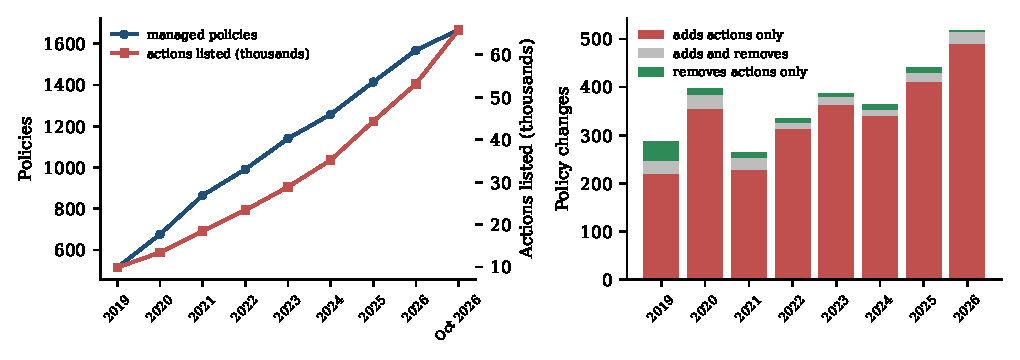
\includegraphics[width=0.85\textwidth]{figures/growth.pdf}
  \caption{Left: managed policies and actions listed. Right: modifications that changed which actions a policy grants, by year and
  direction (neutral changes excluded).}
  \label{fig:growth}
\end{figure*}

\subsection{A one-way ratchet}
\label{sec:ratchet}
Of 11{,}107 modifications, 2{,}992 changed the action patterns a policy grants. Of those, 2{,}723 (91\%) only added patterns, 168 (6\%)
added and removed, and 101 (3\%) only removed. Across all modifications, 28{,}632 patterns were added and 1{,}796 removed, a ratio of 16
to 1. The cohort of 675 policies that existed in June 2020 and still exist grew from 13{,}381 to 26{,}539 listed actions; 43\% of them
grew and 1\% shrank.

The pattern holds in every category (Table~\ref{tab:kind}). Additions were 90\% of substantive changes to customer-attachable policies,
82\% for job-function policies and 93--94\% for service-linked and service-role policies. Job-function policies, which customers attach
to people, had the highest share of removals, but still changed towards more permission four times in five.

\begin{table}[t]
\centering
\caption{Direction of substantive modifications by policy category.}
\label{tab:kind}
\footnotesize
\begin{tabular}{lrrrr}
\toprule
Category & Add & Both & Remove & Add share \\
\midrule
Other (attachable) & 1,521 & 109 & 59 & 90\% \\
Job function & 60 & 8 & 5 & 82\% \\
Service role & 336 & 10 & 11 & 94\% \\
Service-linked & 763 & 37 & 18 & 93\% \\
Since deprecated & 43 & 4 & 8 & 78\% \\
\bottomrule
\end{tabular}
\end{table}


\subsection{Which services}
\label{sec:services}
Added patterns came from 408 services, but a few dominate: EC2 (2{,}016 additions), SageMaker (762), S3 (751), Glue (566), Bedrock (517),
DataZone (423), IAM (415) and Bedrock AgentCore (412). The list mirrors AWS's product priorities over the period: compute and storage
throughout, then machine learning and, from 2023, generative AI and agent services. IAM itself is among the top ten, so managed policies
increasingly grant permissions over identities, not only over resources.

\subsection{Cadence}
\label{sec:cadence}
Substantive changes are concentrated but continual. 815 policies had at least one; the median policy had two and the 90th percentile
seven. \texttt{ReadOnlyAccess} changed 104 times, more than any other policy. The median interval between substantive changes to the same
policy was 90 days. Substantive changes per year rose from 265--397 in 2019--2023 to 441 in 2025 and 518 in the first nine and a half months
of 2026, so the rate at which customers' attached permissions change is increasing.

\subsection{Effective grants and silent growth}
\label{sec:silent}
\begin{table*}[t]
\centering
\caption{Explicit and effective grants, and policies granting permissions-management actions unconditionally on all resources. Effective grants expand every Allow pattern against the actions known (first seen in any managed policy) at the snapshot date. Attachable policies exclude service-linked and service-role policies.}
\label{tab:eff}
\footnotesize
\begin{tabular}{lrrrrrr}
\toprule
Snapshot & Policies & Explicit actions & Effective actions & Ratio & Perm.-mgmt.\ on \texttt{*} & of which attachable \\
\midrule
2020 & 676 & 13,294 & 32,386 & 2.44 & 104 & 62 \\
2021 & 865 & 18,268 & 42,964 & 2.35 & 126 & 76 \\
2022 & 991 & 22,998 & 52,350 & 2.28 & 133 & 80 \\
2023 & 1,140 & 28,317 & 62,653 & 2.21 & 139 & 81 \\
2024 & 1,257 & 34,385 & 75,750 & 2.20 & 148 & 88 \\
2025 & 1,414 & 43,019 & 92,246 & 2.14 & 164 & 101 \\
2026 & 1,568 & 51,454 & 127,297 & 2.47 & 182 & 117 \\
Oct 2026 & 1,667 & 63,870 & 148,941 & 2.33 & 193 & 126 \\
\bottomrule
\end{tabular}
\end{table*}


Wildcards make policies grant far more than they list. Expanded against the actions known at each date, all policies together granted
32{,}386 actions in 2020 and 148{,}941 in October 2026, 2.1--2.5 times the explicit count in every year (Table~\ref{tab:eff},
Fig.~\ref{fig:eff}). For the 675-policy cohort, effective grants rose from 32{,}295 to 69{,}997; 68\% of cohort policies grew in effect and
0.6\% shrank.

Growth did not require edits. Of the cohort, 357 policies had the same default version in 2026 as in 2020. Excluding the two policies
whose action is \texttt{*}, 156 of the remaining 356 nevertheless grew in effect, by an estimated 4{,}748 actions in total, because
their wildcards matched actions that first appeared later, for example \texttt{AmazonEC2FullAccess} (407 to 641) and
\texttt{AWSElasticBeanstalkFullAccess} (782 to 1{,}274). No change event, version bump or changelog entry marks this growth. The
estimate is an upper bound: an action's first appearance in a managed policy can follow its launch. Restricting to the 239 services
that first appeared after June 2020, whose actions cannot have existed earlier, gives a strict lower bound of 204 actions in 15
policies.

\begin{figure*}[t]
  \centering
  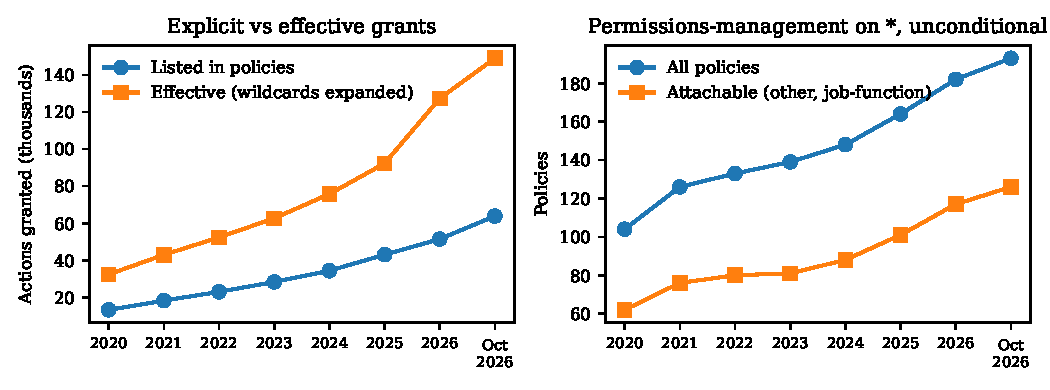
\includegraphics[width=0.85\textwidth]{figures/effective.pdf}
  \caption{Left: total actions listed in Allow statements and effective actions after wildcard expansion. Right: policies granting
  permissions-management actions unconditionally on all resources.}
  \label{fig:eff}
\end{figure*}

\subsection{Resource scope}
\label{sec:scope}
The share of Allow statements on all resources fell from 69\% to 48\%, because recently created policies are scoped more carefully.
Changes to existing policies went the other way: 756 modifications increased the number of statements on \texttt{*} and 58 decreased it.
New policies are better than old ones, but old ones get broader.

\subsection{Privilege escalation and permissions management}
\label{sec:esc}
The narrow escalation screen was stable: 24 policies in 2019 and 24 in 2026. Besides administrator and IAM policies, the set includes the
\texttt{DataScientist} and \texttt{SystemAdministrator} job-function policies, which grant \texttt{lambda:UpdateFunctionCode} on all
functions, enough to run code as any function's execution role. Only four modifications added escalation actions to an existing policy;
three were to \texttt{AdministratorAccess-Amplify} in 2021, which acquired \texttt{iam:AttachRolePolicy}, \texttt{iam:PutRolePolicy},
\texttt{iam:CreatePolicyVersion}, \texttt{iam:PassRole}, \texttt{iam:UpdateAssumeRolePolicy} and \texttt{lambda:UpdateFunctionCode} on
all resources in three steps. Customers who attached it for Amplify development gained the ability to escalate to administrator.

The broader permissions-management screen tells a different story (Table~\ref{tab:eff}). Policies granting such actions unconditionally
on all resources rose from 104 to 193, and customer-attachable ones from 62 to 126. Job-function policies show the same drift:
\texttt{SystemAdministrator} grew from 20 to 34 such actions, \texttt{DatabaseAdministrator} from 5 to 10 (adding, for example,
\texttt{rds:AuthorizeDBSecurityGroupIngress} and \texttt{redshift:AuthorizeDataShare}), and \texttt{DataScientist} from 4 to 12 (adding
\texttt{es:UpdateElasticsearchDomainConfig}, which can change a search domain's access policy). Few of these are direct paths to
administrator, but each lets the holder change who else can reach a resource, and they accumulate in policies that customers attach to
people.

\subsection{What ``read-only'' allows}
\label{sec:ro}
\texttt{ReadOnlyAccess} changed 104 times and its effective grant rose from 1{,}877 actions in 2020 to 6{,}186 in 2026. ``Read-only'' here
means ``does not create, modify or delete resources''; it does not mean ``cannot read data''. In both years it granted 17 of the 20
probed actions, including \texttt{s3:GetObject}, \texttt{dynamodb:GetItem}, \texttt{dynamodb:Query} and \texttt{dynamodb:Scan},
\texttt{ssm:GetParameter} and \texttt{ssm:GetParameters}, \texttt{logs:GetLogEvents}, \texttt{athena:GetQueryResults},
\texttt{codecommit:GetFile}, \texttt{ecr:BatchGetImage} and \texttt{lambda:GetFunction} (which returns a link to the function's code). It
did not grant \texttt{secretsmanager:GetSecretValue} or \texttt{kms:Decrypt}, so secrets and encrypted SecureString parameters stay
protected, but plaintext parameters, objects, table items and logs do not. It also grants \texttt{sqs:ReceiveMessage}, which hides a
message from other consumers for the visibility timeout, and \texttt{kinesis:GetRecords}: a ``read-only'' principal can interfere with a
queue's processing. \texttt{ViewOnlyAccess} granted none of the probed actions, and \texttt{SecurityAudit} only
\texttt{cloudformation:GetTemplate} and \texttt{rds:DownloadDBLogFilePortion}. Customers who need an auditor role should start from
these, not from \texttt{ReadOnlyAccess}.

\subsection{A new pattern: conditional full wildcard}
\label{sec:mcp}
\texttt{AWSMcpServiceActionsFullAccess}, created in November 2025 and updated in February 2026, allows every action on every resource when
the request carries the condition key \texttt{aws:IsMcpServiceAction}. It is one of only two current policies whose action is \texttt{*},
the other being \texttt{AdministratorAccess}, and its arrival explains the jump in effective grants in 2026 (Table~\ref{tab:eff}). Its
safety rests entirely on the semantics and enforcement of a single, new condition key tied to actions taken through an AI-agent tool
interface \cite{mcp2024}. If that key were ever set in requests outside its intended path, the policy would be equivalent to
administrator access.

\section{Discussion}
\label{sec:disc}
Managed policies trade control for convenience, and the trade grows over time. The direction of change is overwhelmingly towards more
permission, which is unsurprising for policies that must keep up with new features, but it means that attaching a managed policy delegates
future permission decisions to AWS. Two mechanisms carry that delegation: explicit edits, which are visible in the archive and in AWS's
policy-update notices, and wildcard expansion, which is not visible anywhere. Customer-side reviews that happen at attachment time see
neither.

\paragraph*{Recommendations}
\begin{enumerate}
\item Treat managed-policy updates as permission changes: subscribe to a change feed (the archive offers one) and review updates to
policies attached in production.
\item Re-evaluate effective permissions periodically, not only policy text; tools that expand wildcards against the current action list
reveal silent growth.
\item Prefer customer-managed copies for sensitive principals, accepting the maintenance cost, and avoid service wildcards in them.
\item Check job-function policies for escalation and permissions-management actions before using them as defaults for people.
\item Use \texttt{ViewOnlyAccess} or \texttt{SecurityAudit}, not \texttt{ReadOnlyAccess}, for principals that must not read data.
\item Scrutinise conditional wildcards: a condition key is a single point of failure.
\end{enumerate}

\paragraph*{Threats to validity}
The archive records default versions only, from February 2019, and its early months were built incrementally, so 2019 figures
under-count. Pattern-level comparison of changes overstates churn when explicit lists are replaced by wildcards. The action registry
records the first appearance of an action in a managed policy, not its launch, and covers only actions that some managed policy has
listed explicitly; effective counts are therefore approximate, which is why we report bounds for silent growth. The security screens
ignore scoped and conditional grants and combinations, and access levels come from a community-maintained copy of AWS documentation
\cite{iamdataset}. Finally, we do not know how often each policy is attached, so we cannot weight findings by exposure.

\section{Conclusion}
Over seven years, changes to AWS managed policies almost always added permissions: 91\% of substantive modifications only added, grants
added outnumbered grants removed sixteen to one, and the pattern held in every category. Wildcards add a second, invisible channel of
growth. Policies that customers attach to people accumulated permissions-management actions, and the policy named ``read-only'' reads
customer data. Customers should treat attached managed policies as permissions that change under them.

\section*{Data availability}
The archive is public \cite{mamip}. Analysis code and results are available at
\url{https://github.com/mithil2k2000-tech/aws-managed-policy-drift} and archived at \url{https://doi.org/10.5281/zenodo.23593032}.

\section*{Declaration of generative AI use}
The author used Claude (Anthropic) to help write analysis code and draft text. The author designed the study, reviewed the code, results
and text, and takes full responsibility for the content.

\section*{Conflict of interest}
The author declares no conflict of interest. This work received no specific funding.

\bibliographystyle{IEEEtran}
\bibliography{refs}

\end{document}
